%------------------------------------------------------------------------------
\chapter{Scaled multijet MC distributions}
\label{sec:app2}
%------------------------------------------------------------------------------
In this appendix, the data/bkg.\ comparison plots for two kinematic variables are shown, in which the multijet background is considered from both the multijet MC and the scaled multijet MC (as described in \ref{sec:abcd:furtherimprovement:scaledcorr}) and the other backgrounds are from the MC simulation.

Fig.\ \ref{fig:app:ab:vlqm} and Fig.\ \ref{fig:app:cd:vlqm} show the VLQ mass distribution in all the four regions A, B, C and D when the likelihood fit is performed on region A, B together and region C, D together. These distributions show both the multijet MC (which are mismodelled) and the scaled multijet MC.

Fig.\ \ref{fig:app:ab:ljetpt} and Fig.\ \ref{fig:app:cd:ljetpt} show the \pt distribution of $W$-tagged jet in all the four regions A, B, C and D when the likelihood fit is performed on region A, B together and region C, D together. These distributions show both the multijet MC (which are mismodelled) and the scaled multijet MC.

\begin{figure}[hbt!]
	\centering
	\graphicspath{{figs/appendix/scaledmultijet/ABVLQM/}}
	\begin{subfigure}{.35\textwidth}
		\centering
		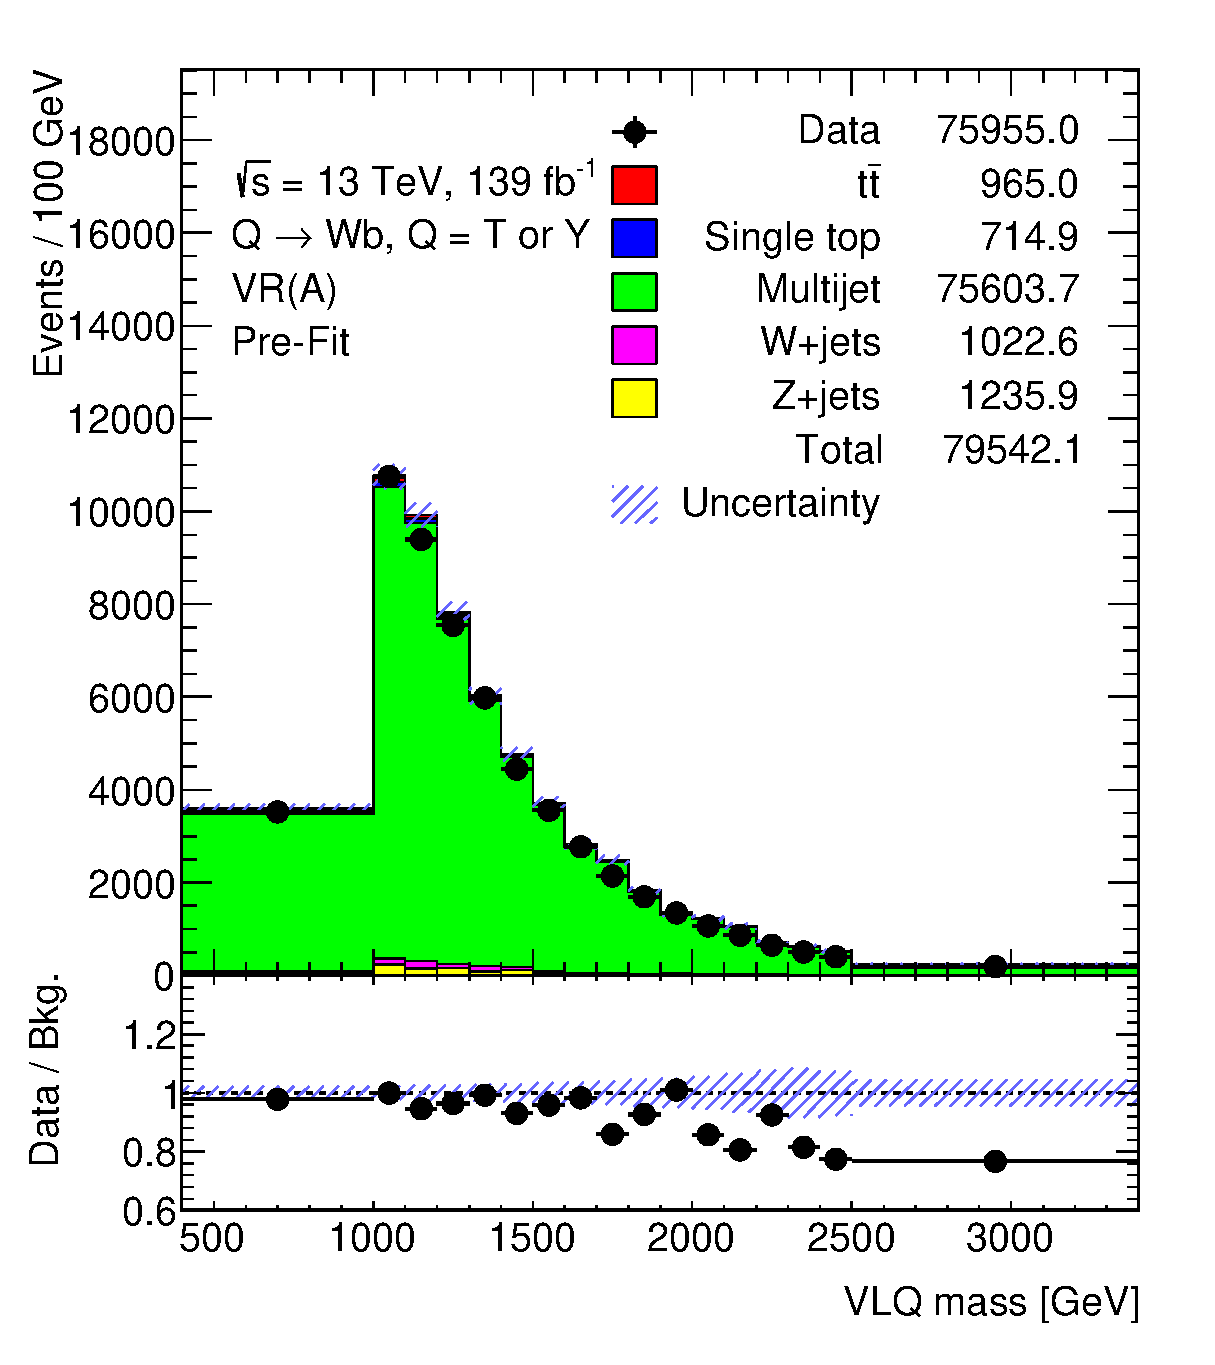
\includegraphics[width=\linewidth,height=\textheight,keepaspectratio]{VR_A_VLQM.eps}
		\caption{}
	\end{subfigure}\hspace{0.6cm}
	\begin{subfigure}{.35\textwidth}
		\centering
		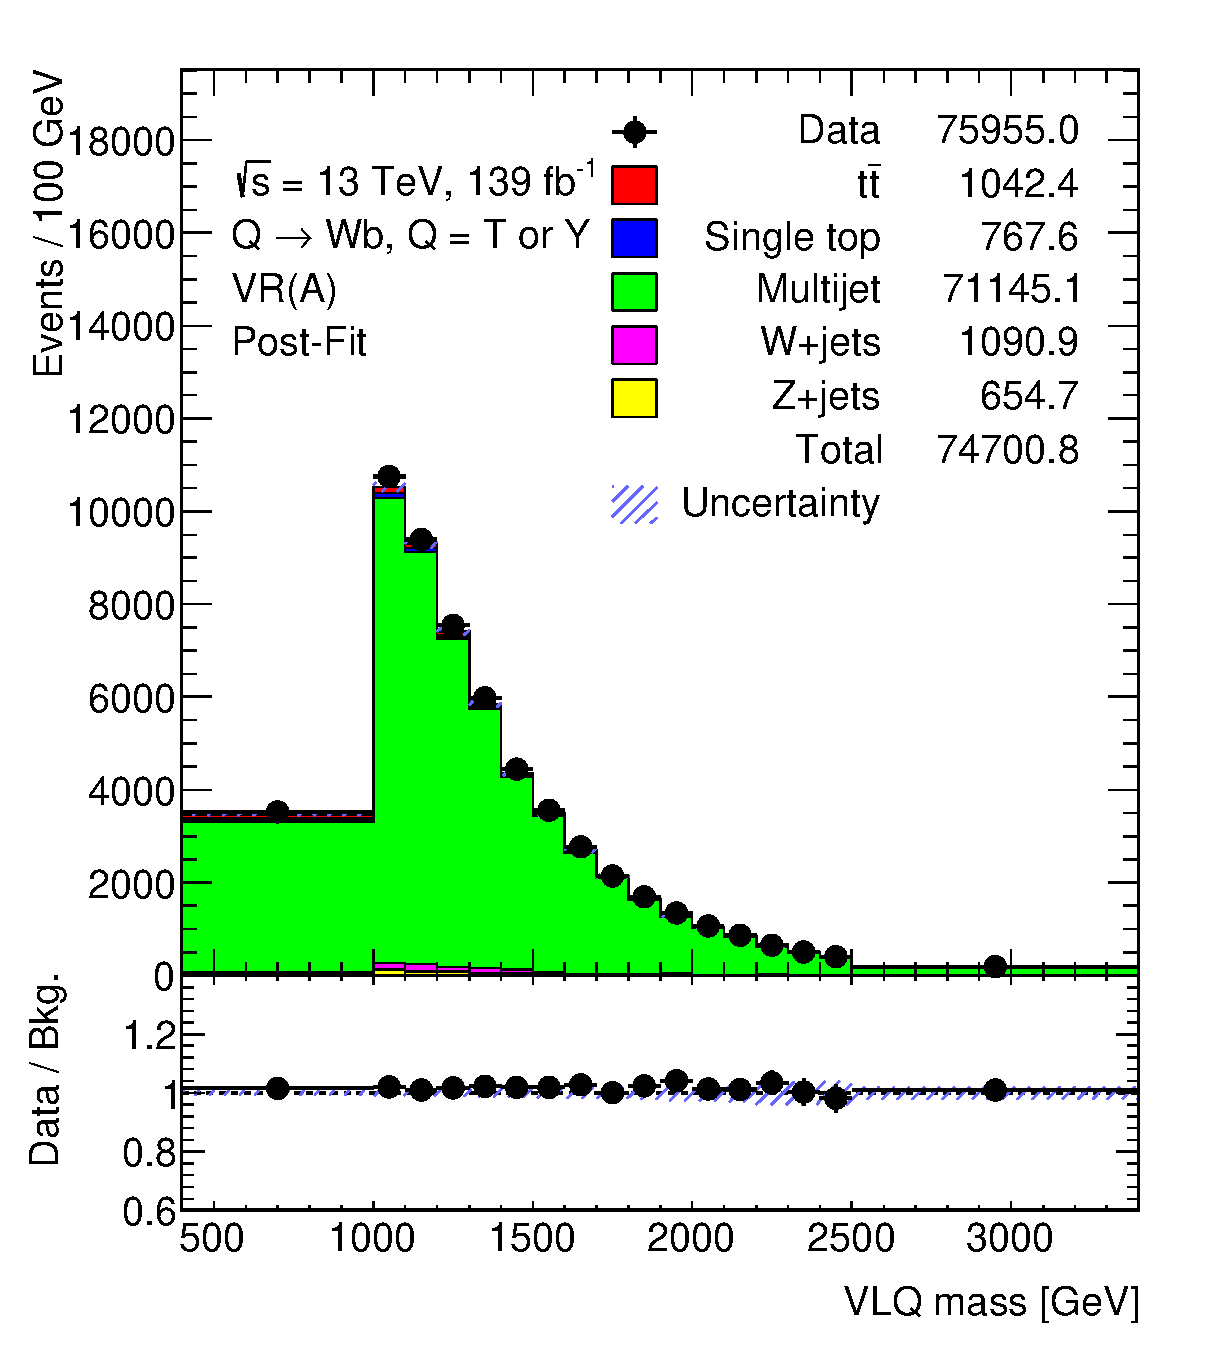
\includegraphics[width=\linewidth,height=\textheight,keepaspectratio]{VR_A_VLQM_postFit.eps}
		\caption{}
	\end{subfigure}
	\begin{subfigure}{.35\textwidth}
		\centering
		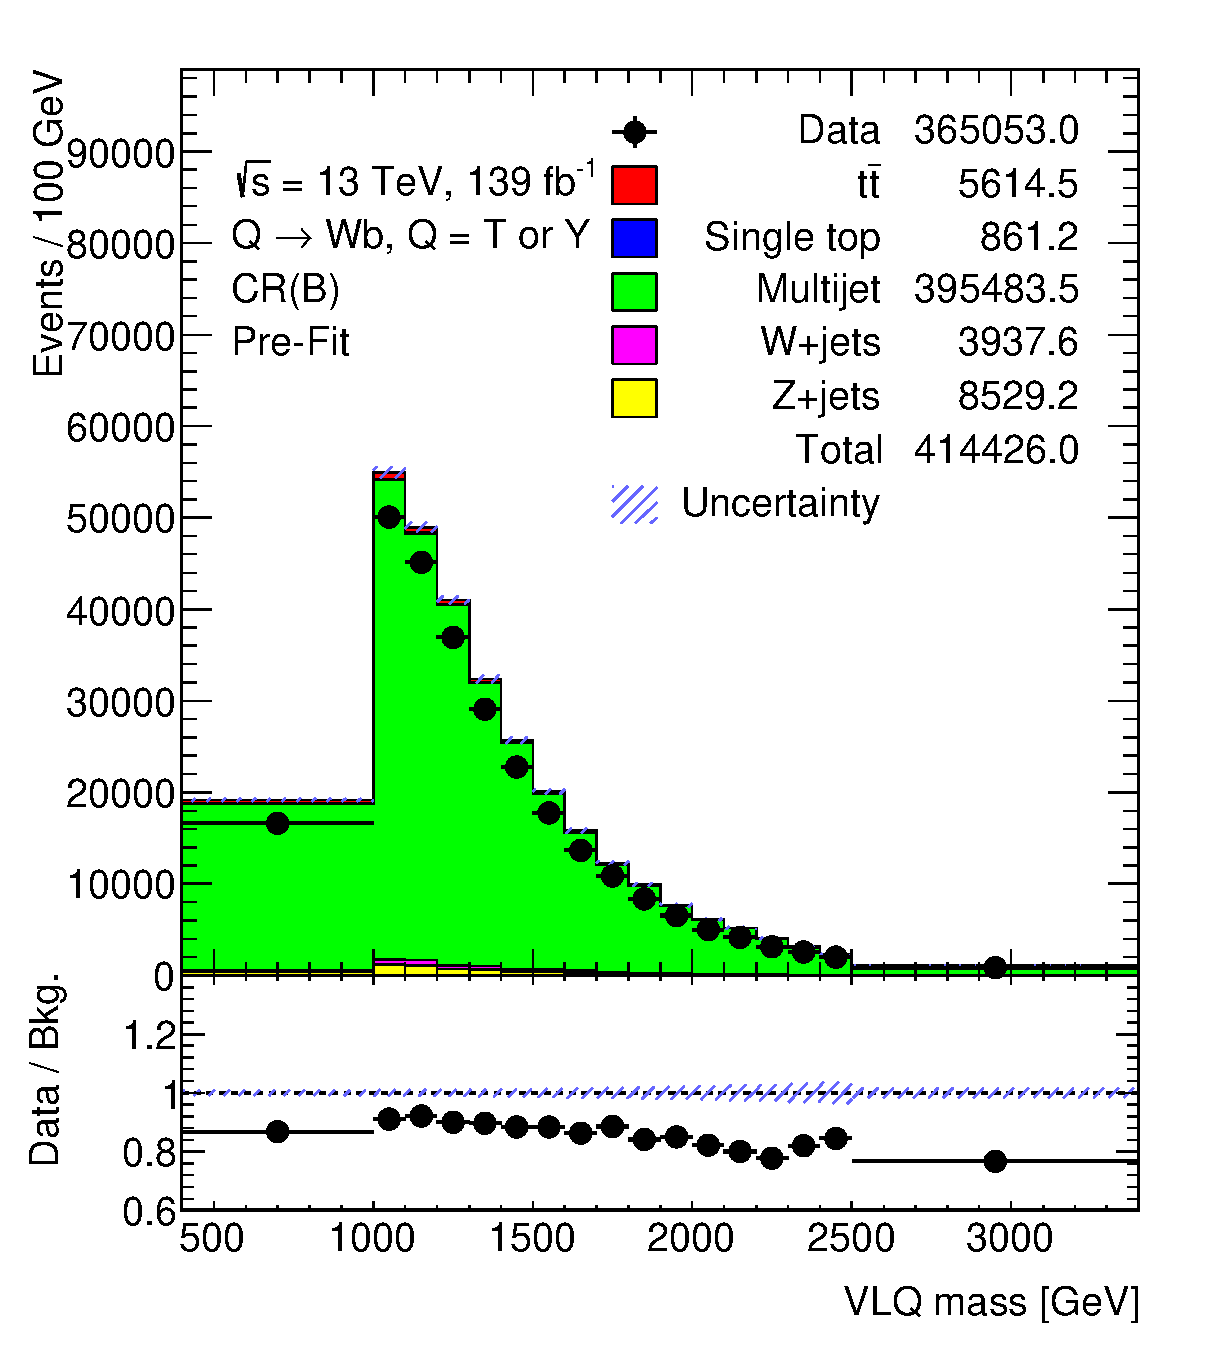
\includegraphics[width=\linewidth,height=\textheight,keepaspectratio]{CR_B_VLQM.eps}
		\caption{}
	\end{subfigure}\hspace{0.6cm}
	\begin{subfigure}{.35\textwidth}
		\centering
		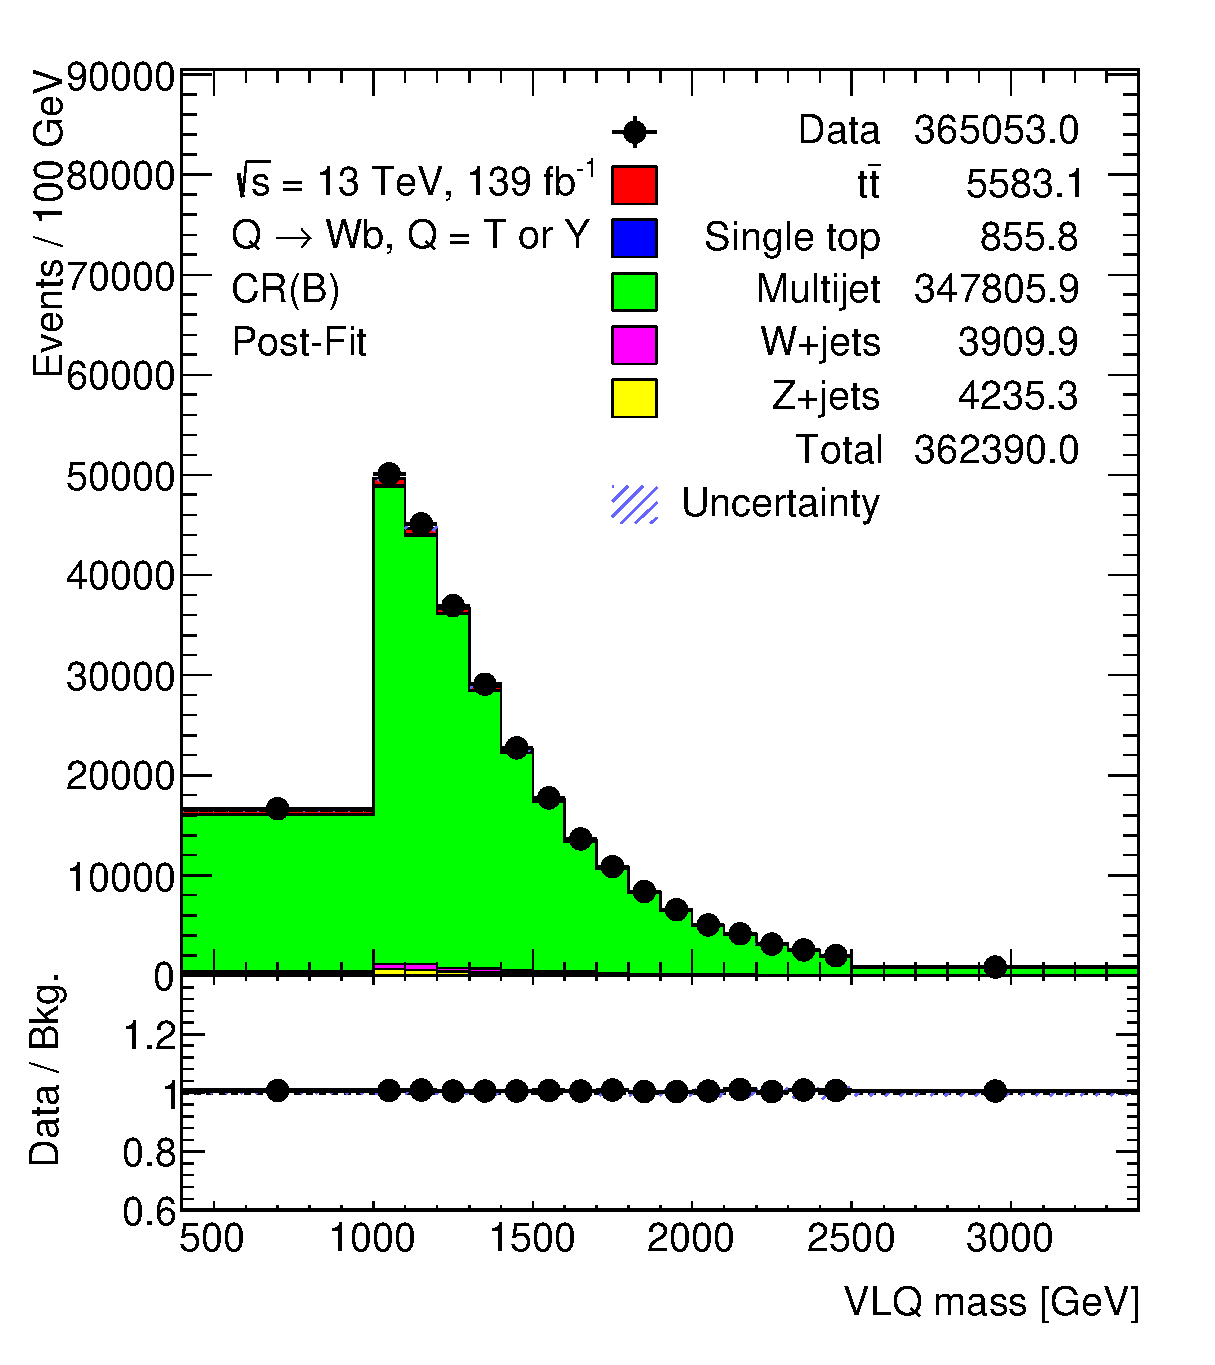
\includegraphics[width=\linewidth,height=\textheight,keepaspectratio]{CR_B_VLQM_postFit.eps}
		\caption{}
	\end{subfigure}
	\caption{VLQ mass distribution is shown when a likelihood fit is performed to fit regions A and B together in which the multijet MC is fitted to the data. It shows the VLQ mass distribution for (a) multijet MC and (b) scaled multijet MC in region A, and (c) multijet MC and (d) scaled multijet MC in region B.}
	\label{fig:app:ab:vlqm}
\end{figure}



\begin{figure}[hbt!]
	\centering
	\graphicspath{{figs/appendix/scaledmultijet/CDVLQM/}}
	\begin{subfigure}{.35\textwidth}
		\centering
		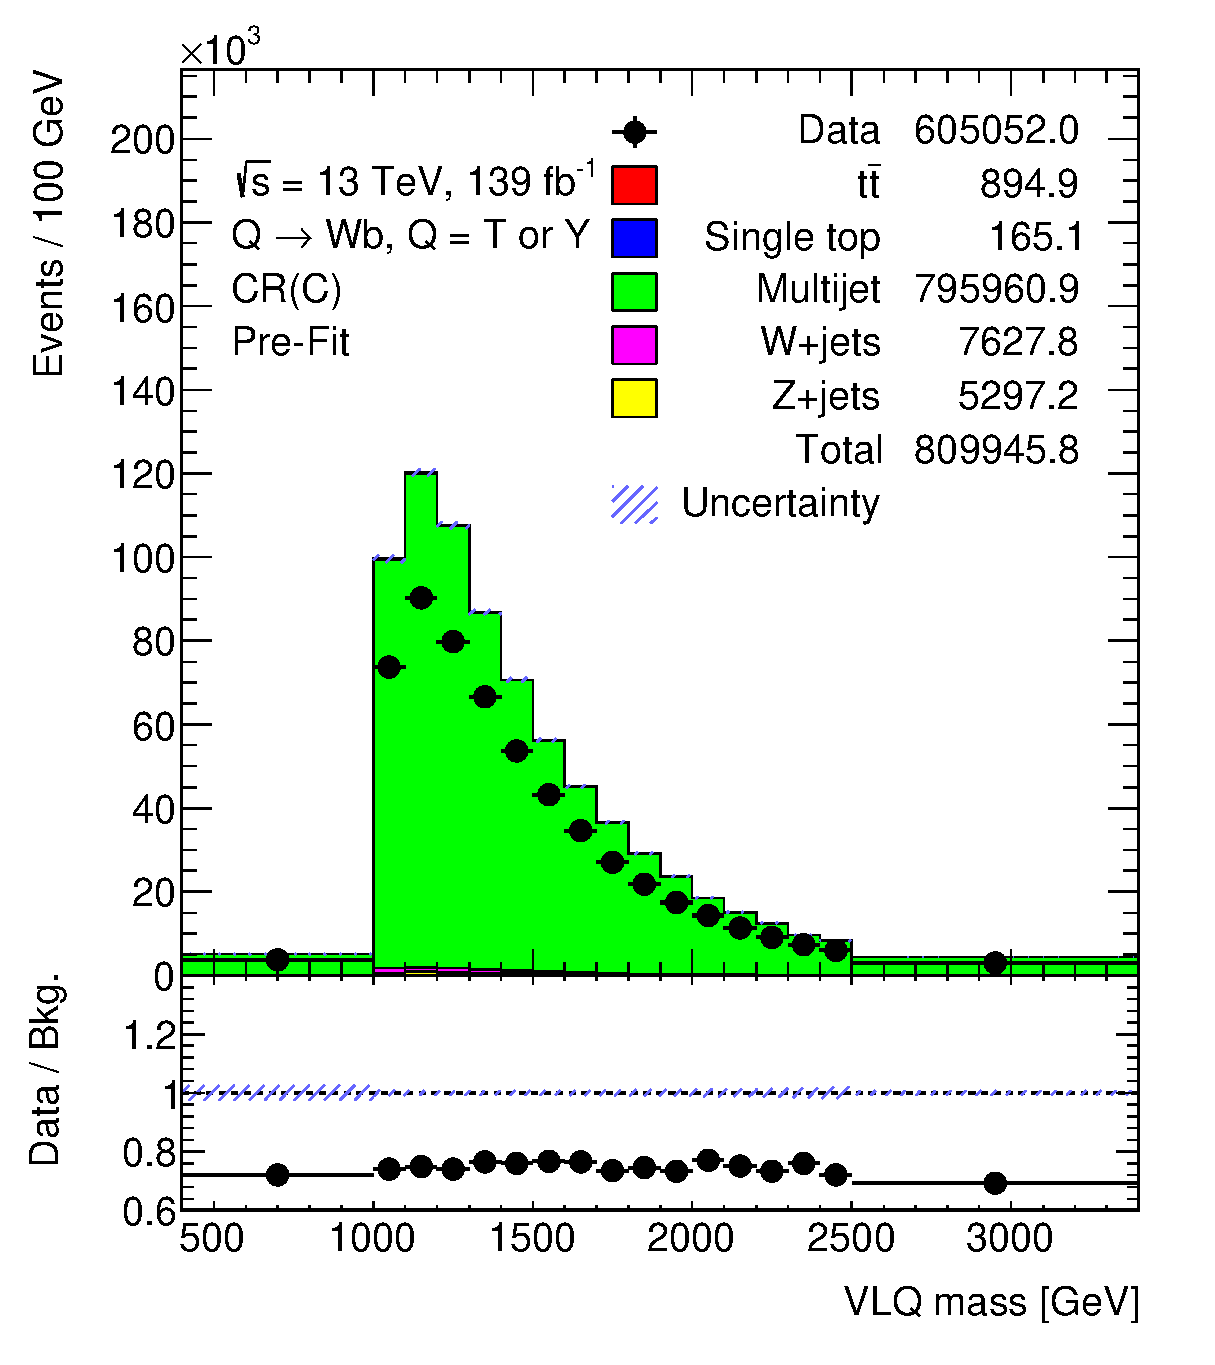
\includegraphics[width=\linewidth,height=\textheight,keepaspectratio]{CR_C_VLQM.eps}
		\caption{}
	\end{subfigure}\hspace{0.6cm}
	\begin{subfigure}{.35\textwidth}
		\centering
		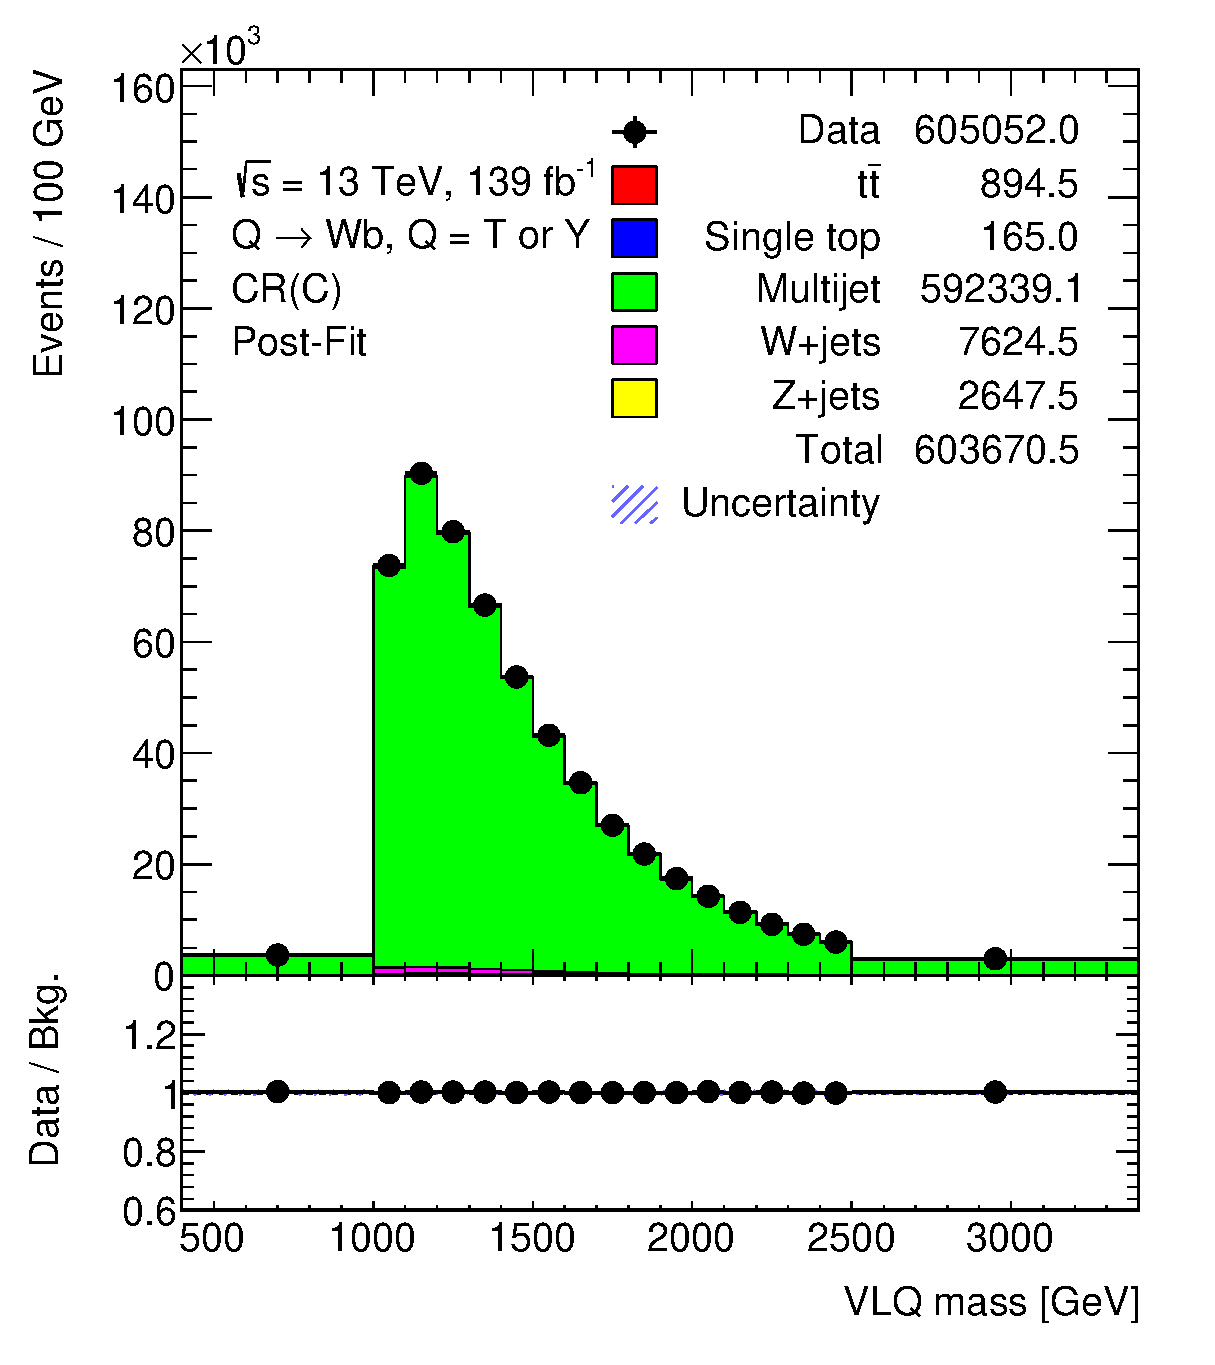
\includegraphics[width=\linewidth,height=\textheight,keepaspectratio]{CR_C_VLQM_postFit.eps}
		\caption{}
	\end{subfigure}
	\begin{subfigure}{.35\textwidth}
		\centering
		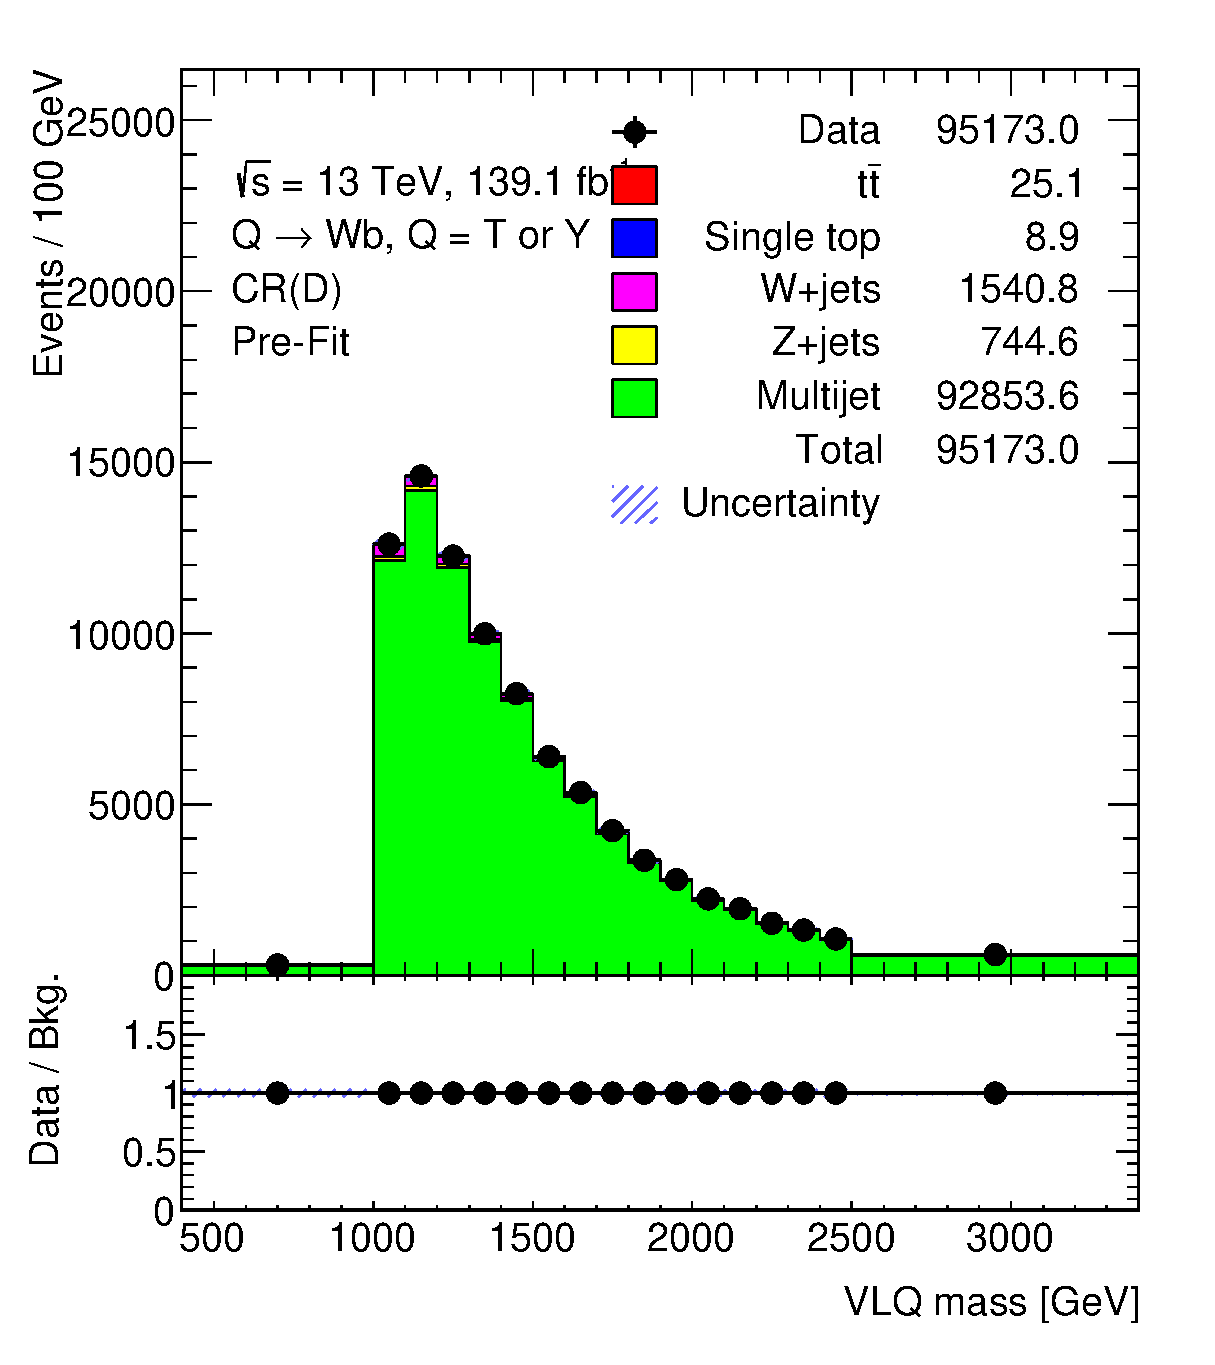
\includegraphics[width=\linewidth,height=\textheight,keepaspectratio]{CR_D_VLQM.eps}
		\caption{}
	\end{subfigure}\hspace{0.6cm}
	\begin{subfigure}{.35\textwidth}
		\centering
		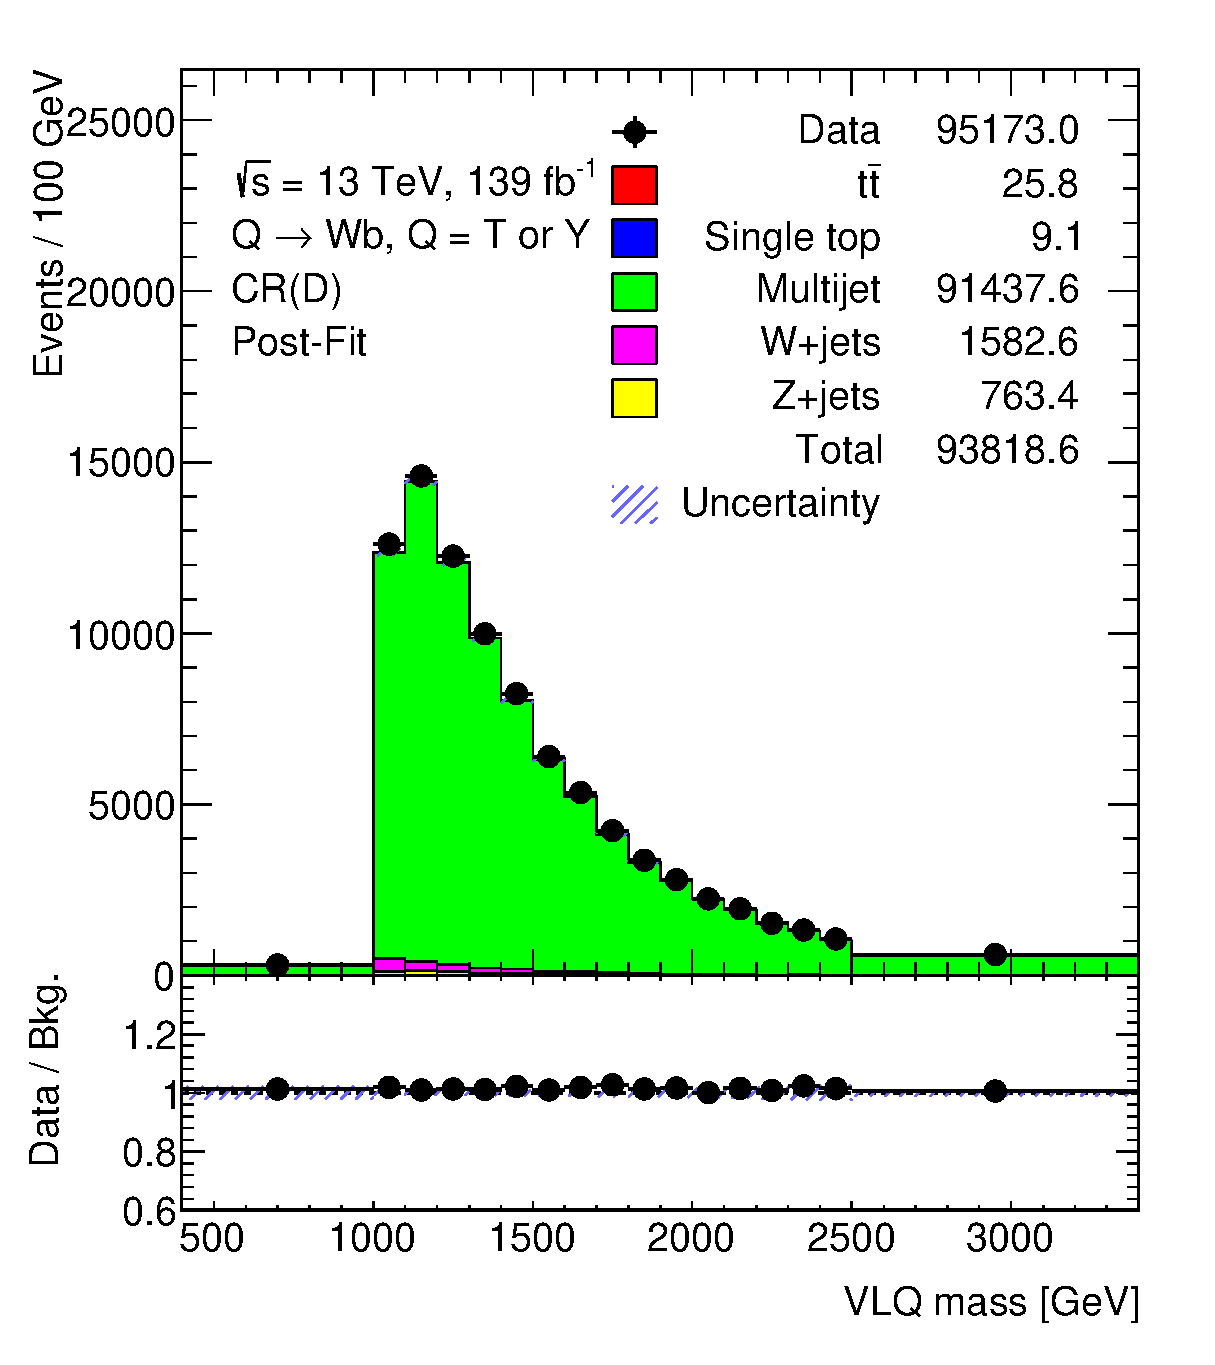
\includegraphics[width=\linewidth,height=\textheight,keepaspectratio]{CR_D_VLQM_postFit.eps}
		\caption{}
	\end{subfigure}
	\caption{VLQ mass distribution is shown when a likelihood fit is performed to fit regions C and D together in which the multijet MC is fitted to the data. It shows the VLQ mass distribution for (a) multijet MC and (b) scaled multijet MC in region C, and (c) multijet MC and (d) scaled multijet MC in region D.}
	\label{fig:app:cd:vlqm}
\end{figure}



\begin{figure}[hbt!]
	\centering
	\graphicspath{{figs/appendix/scaledmultijet/ABljetpt/}}
	\begin{subfigure}{.35\textwidth}
		\centering
		\includegraphics[width=\linewidth,height=\textheight,keepaspectratio]{VR_A_ljet_pt.eps}
		\caption{}
	\end{subfigure}\hspace{0.6cm}
	\begin{subfigure}{.35\textwidth}
		\centering
		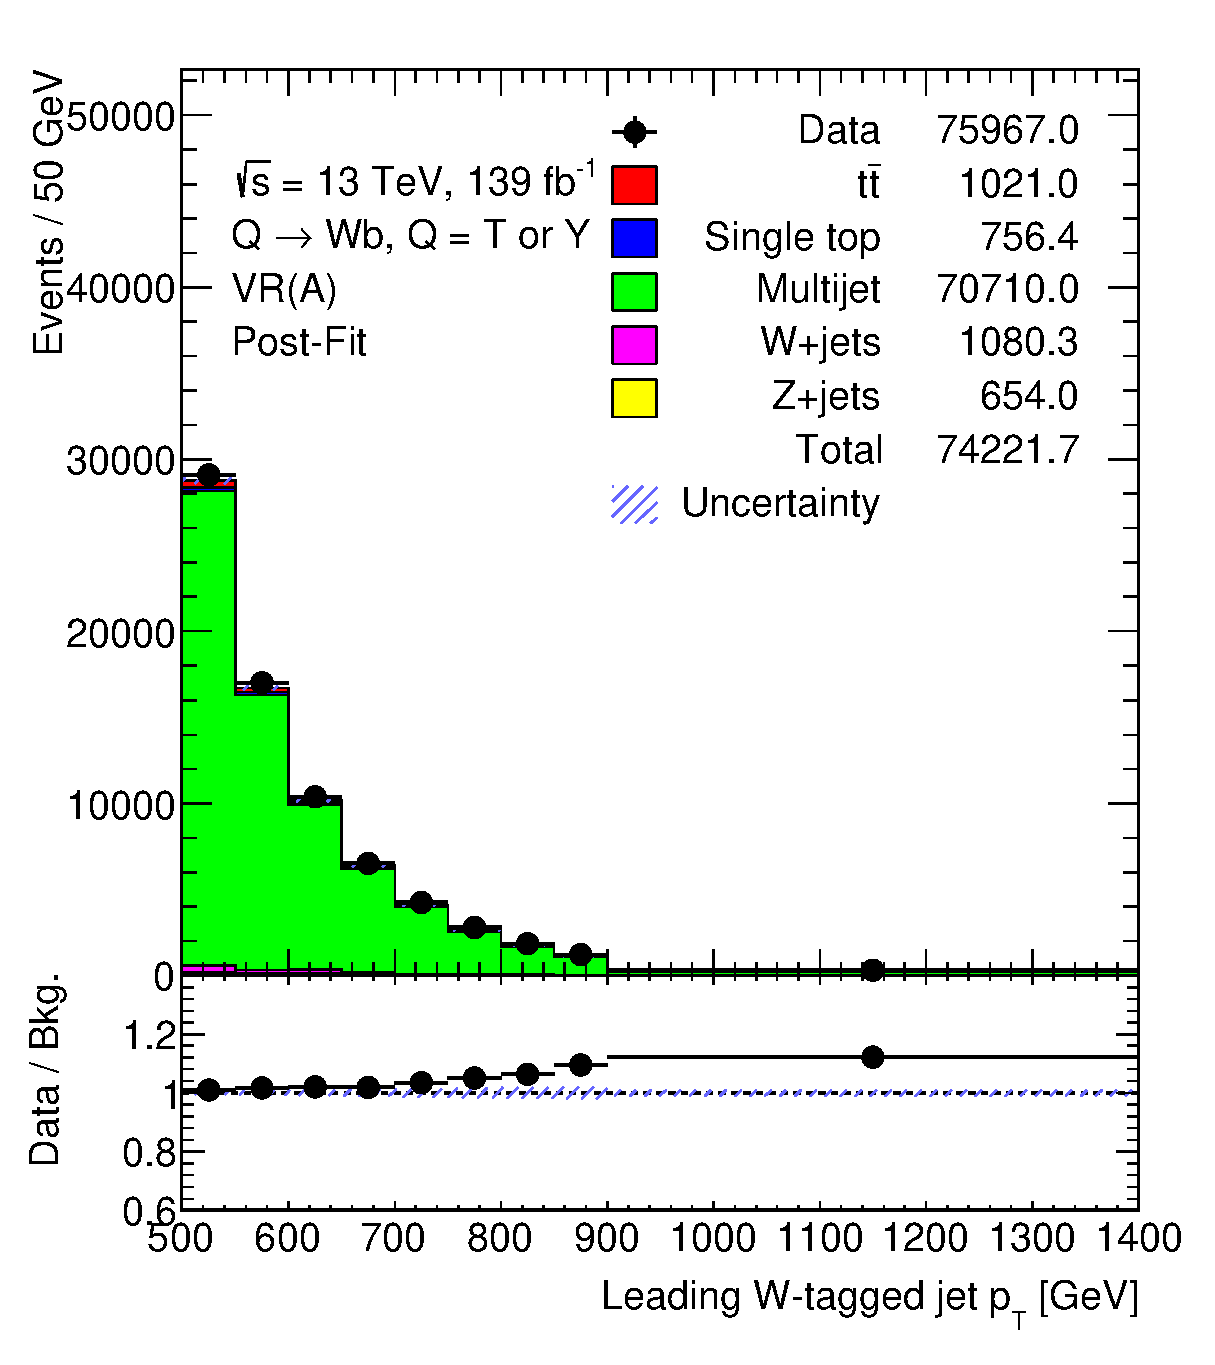
\includegraphics[width=\linewidth,height=\textheight,keepaspectratio]{VR_A_ljet_pt_postFit.eps}
		\caption{}
	\end{subfigure}
	\begin{subfigure}{.35\textwidth}
		\centering
		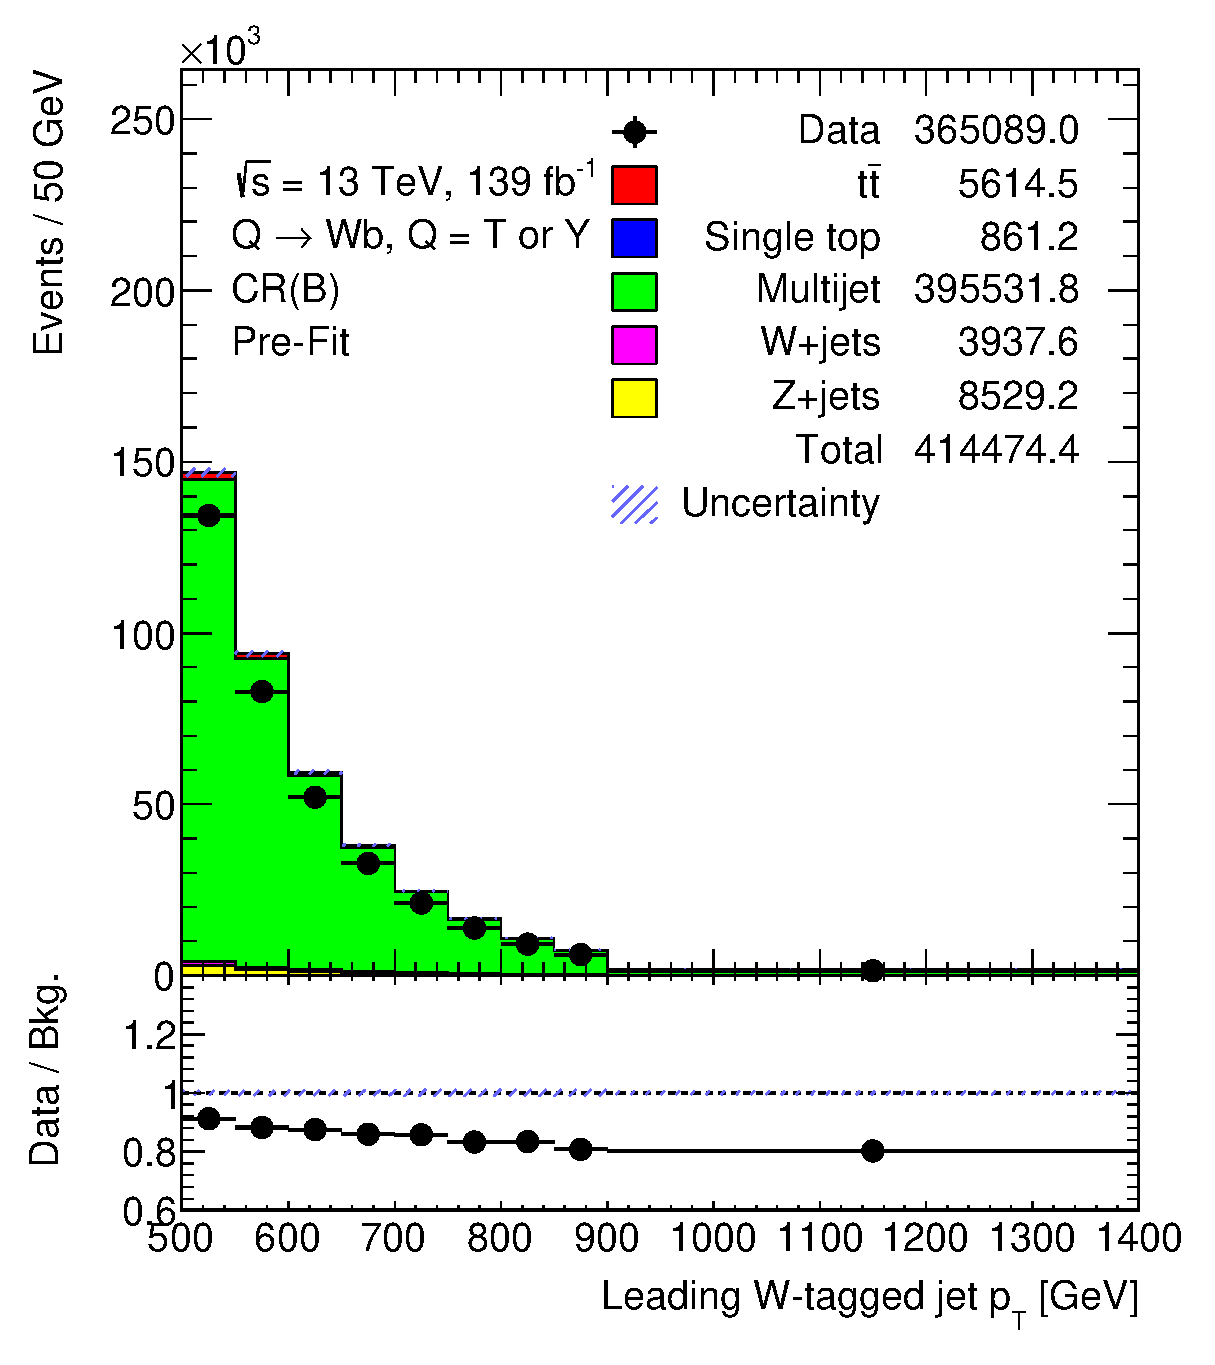
\includegraphics[width=\linewidth,height=\textheight,keepaspectratio]{CR_B_ljet_pt.eps}
		\caption{}
	\end{subfigure}\hspace{0.6cm}
	\begin{subfigure}{.35\textwidth}
		\centering
		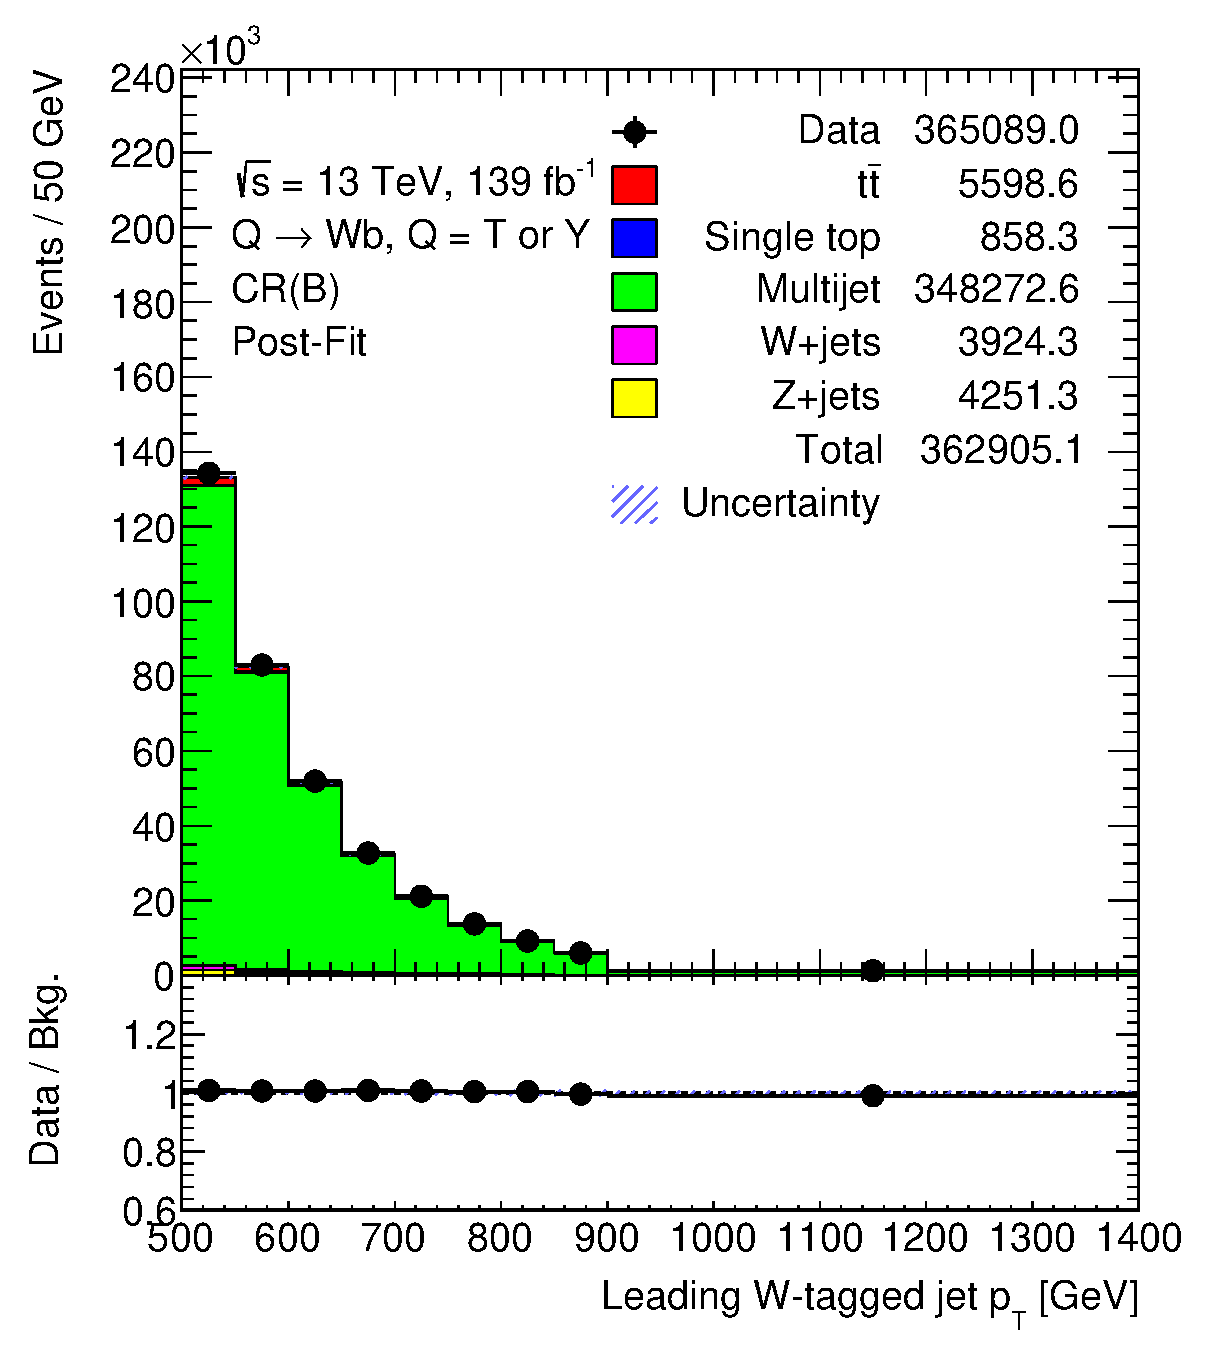
\includegraphics[width=\linewidth,height=\textheight,keepaspectratio]{CR_B_ljet_pt_postFit.eps}
		\caption{}
	\end{subfigure}
	\caption{\pt distribution of $W$-tagged jet is shown when a likelihood fit is performed to fit regions A and B together in which the multijet MC is fitted to the data. It shows \pt distribution of $W$-tagged jet for (a) multijet MC and (b) scaled multijet MC in region A, and (c) multijet MC and (d) scaled multijet MC in region B.}
	\label{fig:app:ab:ljetpt}
\end{figure}



\begin{figure}[hbt!]
	\centering
	\graphicspath{{figs/appendix/scaledmultijet/CDljetpt/}}
	\begin{subfigure}{.35\textwidth}
		\centering
		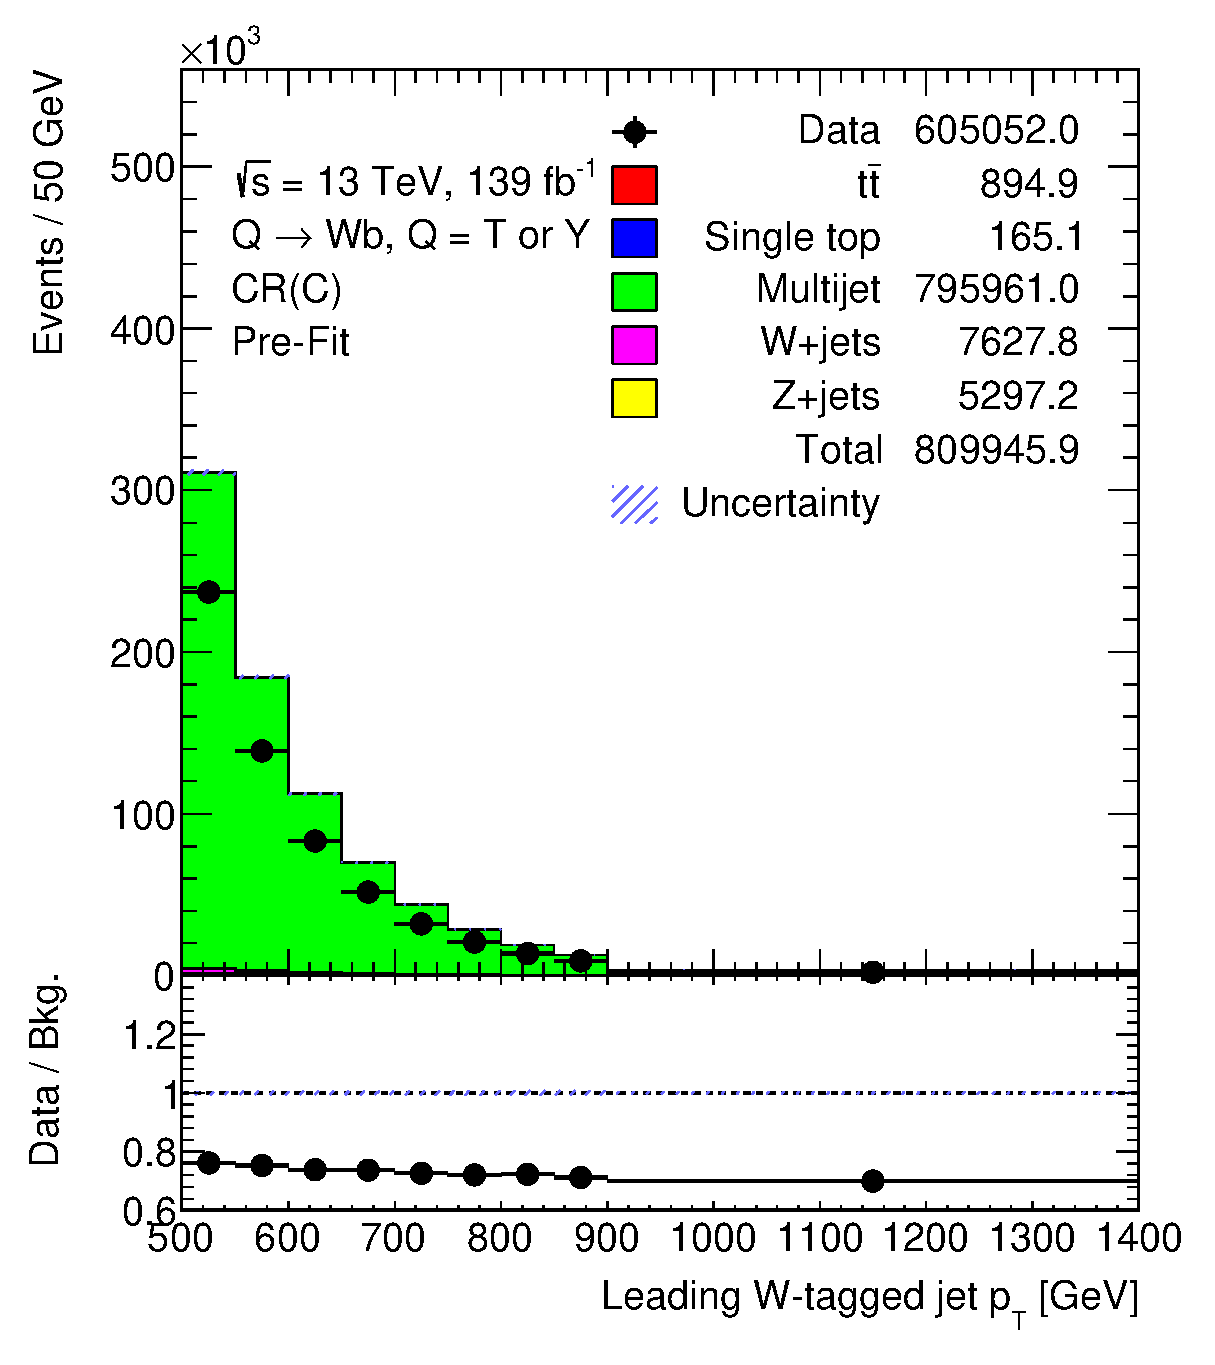
\includegraphics[width=\linewidth,height=\textheight,keepaspectratio]{CR_C_ljet_pt.eps}
		\caption{}
	\end{subfigure}\hspace{0.6cm}
	\begin{subfigure}{.35\textwidth}
		\centering
		\includegraphics[width=\linewidth,height=\textheight,keepaspectratio]{CR_C_ljet_pt_postFit.eps}
		\caption{}
	\end{subfigure}
	\begin{subfigure}{.35\textwidth}
		\centering
		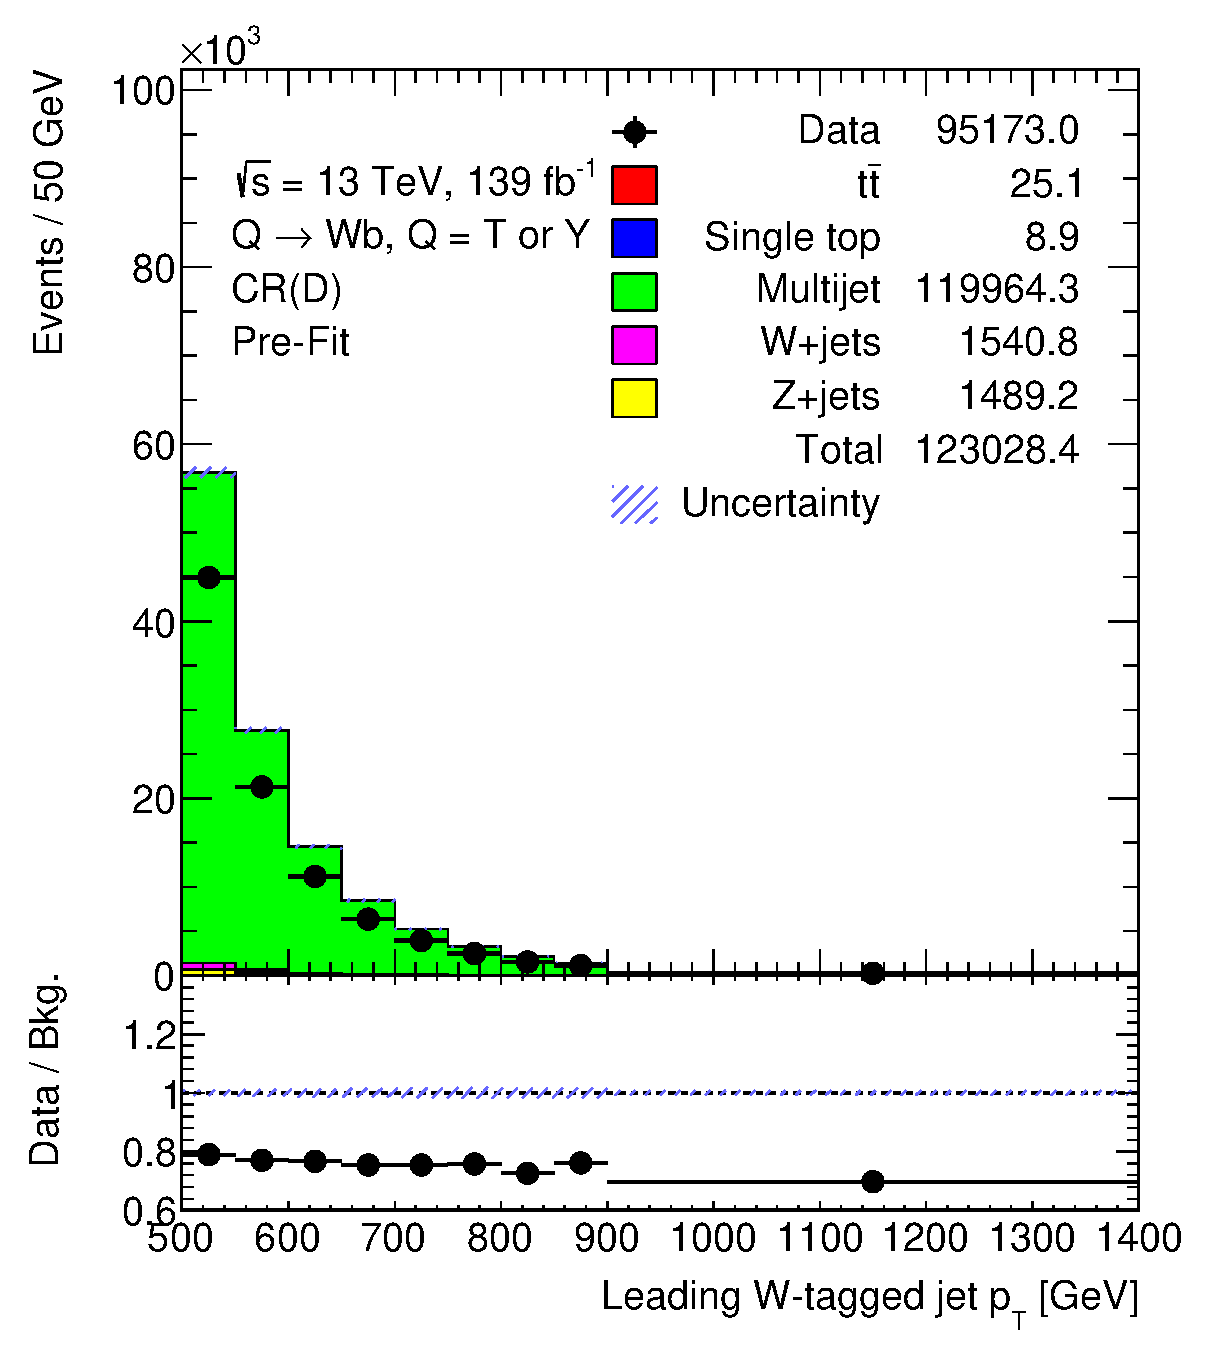
\includegraphics[width=\linewidth,height=\textheight,keepaspectratio]{CR_D_ljet_pt.eps}
		\caption{}
	\end{subfigure}\hspace{0.6cm}
	\begin{subfigure}{.35\textwidth}
		\centering
		\includegraphics[width=\linewidth,height=\textheight,keepaspectratio]{CR_D_ljet_pt_postFit.eps}
		\caption{}
	\end{subfigure}
	\caption{\pt distribution of $W$-tagged jet is shown when a likelihood fit is performed to fit regions C and D together in which the multijet MC is fitted to the data. It shows \pt distribution of $W$-tagged jet for (a) multijet MC and (b) scaled multijet MC in region C, and (c) multijet MC and (d) scaled multijet MC in region D.}
	\label{fig:app:cd:ljetpt}
\end{figure}


%%% Local Variables: 
%%% mode: latex
%%% TeX-master: "../mythesis"
%%% End: 
